\documentclass[11pt,letterpaper]{article}
\usepackage[margin=2cm,includefoot]{geometry}
\usepackage[spanish]{babel}
\usepackage{graphicx}

%%%%% Lenguajes
\newcommand{\pl}{\textsc{Prolog}}
\newcommand{\hsk}{\textsc{Haskell}}
\newcommand{\coql}{\textsc{Coq}}

%%%%%
\renewcommand{\H}{\mathcal{H}}
\newcommand{\B}{\mathcal{B}}
\renewcommand{\S}{\mathcal{S}}
\newcommand{\R}{\mathcal{R}}
\newcommand{\T}{\mathcal{T}}

%%%%% Simbolos logicos
\newcommand{\true}{\mathop{\mathsf{true}}}
\newcommand{\E}{\ensuremath{\exists}}

\newcommand{\dy}{\vee}
\newcommand{\cj}{\wedge}
\newcommand{\imp}{\rightarrow}
\newcommand{\Imp}{\Rightarrow}
\renewcommand{\iff}{\leftrightarrow}
\newcommand{\Iff}{\Leftrightarrow}
\newcommand{\syss}{\leftrightarrow}

\newcommand{\fa}{\forall}
\newcommand{\ex}{\exists}

\newcommand{\G}{\Gamma}
\newcommand{\D}{\Delta}
\newcommand{\Lb}{\Lambda}
\newcommand{\Om}{\Omega}

\newcommand{\lb}{\lambda}
\newcommand{\al}{\alpha}
\newcommand{\ga}{\gamma}

\newcommand{\bool}{\mathsf{Bool}}
\newcommand{\propo}{\ensuremath{\mathsf{PROP}}}
\newcommand{\atom}{\ensuremath{\mathsf{ATOM}}}
\newcommand{\term}{\ensuremath{\mathsf{TERM}}}
\newcommand{\form}{\ensuremath{\mathsf{FORM}}}

\newcommand{\vars}{\ensuremath{\mathsf{Var}}}
\newcommand{\Var}{\ensuremath{\mathsf{Var}}}

\newcommand{\vphi}{\varphi}
\newcommand{\vp}{\varphi}


%%%%% Sustitucion
\newcommand{\sust}[2]{[#1 := #2]}

%alpha equivalencia 
\newcommand{\aeq}{\;\;\sim_\al\;\;}

%%%%% Programacion logica
\newcommand{\pmi}{\leftarrow}

\newcommand{\impp}{\ensuremath{\,\text{:-}\,}\,}
\newcommand{\meta}{\ensuremath{\;\text{?-}\;}}
\newcommand{\si}{\sigma}

\renewcommand{\P}{\mathbb{P}}


%%%%% Razonamiento ecuacional

% \renewcommand{\P}{\mathcal{P}}

\newcommand{\J}{\mathcal{J}}
\newcommand{\hip}[2]{#1:#2}

\newcommand{\eqdef}{=_{def}}

\newcommand{\pf}[2]{#1\vdash#2}
\newcommand{\bk}[2]{#1\vdash_{\bkc}#2}
\newcommand{\bkd}[2]{#1\vdash_{\bkdc}#2}
\newcommand{\tcp}[2]{#1\vdash_{C}#2} %??

\newcommand{\bkc}{\mathcal{B}}
\newcommand{\bkdc}{\mathcal{B}^{\textsc{Dem}}}

%%%%% Deduccion natural
\newcommand{\dn}{\mathsf{DN}}
\newcommand{\dnC}{\mathsf{DN_C}}
\newcommand{\dnM}{\mathsf{DN_M}}
\newcommand{\dnp}{\mathsf{DN_p}}
\newcommand{\dnm}{\mathsf{DN_p^M}}
\newcommand{\dnc}{\mathsf{DN_p^C}}

\newcommand{\Dnm}{\mathsf{DN_m}}
\newcommand{\Dni}{\mathsf{DN_i}}
\newcommand{\Dnc}{\mathsf{DN_c}}
%\newcommand{\dnp}{\mathsf{DN}}
% \renewcommand{\vp}{A}
% \renewcommand{\psi}{B}
% \renewcommand{\chi}{C}


%%%%% Resolucion binaria
\newcommand{\cv}{\Box}
\newcommand{\sat}{\textsf{SAT}}
\newcommand{\modsrch}{\models_?}



%%%%% Simbolos matematicos

\newcommand{\inc}{\subseteq}
\newcommand{\iso}{\ensuremath{\cong}}
\newcommand{\union}{\ensuremath{\cup}}
\newcommand{\morinyec}{\ensuremath{\precapprox}}
\newcommand{\nin}{\ensuremath{\notin}}
\newcommand{\niso}{\ensuremath{\not \cong}}

\newcommand{\restr}[2]{#1\!\!\boldsymbol{\restriction}\!#2}

\newcommand{\vacio}{\varnothing}
\newcommand{\ol}[1]{\overline{#1}}

\newcommand{\supc}{\supseteq}
\newcommand{\limo}{\mathop{\mathpzc{Lim}}}
\newcommand{\ord}{\mathsf{OR}}


\newcommand{\vx}{\vec{x}}
\newcommand{\vy}{\vec{y}}
\newcommand{\vz}{\vec{z}}
\newcommand{\vt}{\vec{t}}
\newcommand{\vf}{\vec{f}}

%%%%% Curry-Howard
% \newcommand{\true}{\mathsf{true}}
\newcommand{\false}{\mathsf{false}}
\newcommand{\ifte}[3]{\mathsf{if\;}#1\mathsf{\; then\;}#2\mathsf{\;
    else\;}#3}
\newcommand{\iszero}{\mathop{\mathsf{iszero}}}
%\newcommand{\suc}{\mathop{\mathsf{succ}}}
\newcommand{\pred}{\mathop{\mathsf{pred}}}
\newcommand{\suc}{\mathop{{\sf suc}}}
\newcommand{\no}{\mathop{{\sf not}}}
\newcommand{\fun}{\mathop{{\sf  fun}}}
\newcommand{\inl}{\mathop{{\sf inl }}}
\newcommand{\inr}{\mathop{{\sf inr }}}
\newcommand{\nat}{\mathsf{Nat}}
\newcommand{\Tf}{\mathsf{T}}

\newcommand{\Lp}{{\tt fst}}
\newcommand{\Rp}{{\tt snd}}

\newcommand{\ejp}{\mathop{\mathtt{ejp}}}
\newcommand{\ej}{\mathop{\mathtt{ej}}}
\newcommand{\comp}{\mathop{\mathtt{comp}}}
\newcommand{\eval}{\mathop{\mathtt{eval}}}
\newcommand{\ap}{\mathop{\mathtt{+\!\!\!+}}}


%%%%% Identificadores

\newcommand{\A}{\mathcal{A}}
% \newcommand{\Q}{\ensuremath{\mathbb{Q}}}
% \newcommand{\Z}{\ensuremath{\mathbb{Z}}}
% \newcommand{\N}{\ensuremath{\mathbb{N}}}
% \newcommand{\R}{\ensuremath{\mathbb{R}}}

\newcommand{\F}{\mathcal{F}}
\newcommand{\Ge}{\mathcal{G}}
\newcommand{\Pe}{\mathcal{P}}
\newcommand{\I}{\mathcal{I}}
\newcommand{\C}{\mathcal{C}}
\newcommand{\K}{\mathcal{K}}
\newcommand{\Kb}{\mathbb{K}}
\newcommand{\Eb}{\mathbb{E}}
\newcommand{\Ebs}{\mathbb{E}^\star}
\newcommand{\Ob}{\mathbb{O}}
\newcommand{\Ib}{\mathbb{I}}
\newcommand{\kb}{\bbkappa}
\newcommand{\M}{\mathcal{M}}
\newcommand{\Nc}{\mathcal{N}}
%\newcommand{\E}{\mathcal{E}}
%\newcommand{\R}{\mathcal{R}}
%\newcommand{\Q}{\mathcal{Q}}
\newcommand{\Sc}{\mathcal{S}}
\newcommand{\Sf}{\mathsf{\Sigma}}
\renewcommand{\S}{\mathbb{\Sigma}}
\newcommand{\Te}{\mathcal{T}}
\newcommand{\Rb}{\mathbb{R}}
\newcommand{\Qb}{\mathbb{Q}}
\newcommand{\Kbb}{\mathbb{K}}
% \newcommand{\T}{\mathbb{\Theta}}
\renewcommand{\L}{\mathcal{L}}


\newcommand{\Db}{\mathbb{D}}
\newcommand{\Fb}{\mathbb{F}}
\newcommand{\De}{\mathcal{D}}

\newcommand{\mg}{\mathbb{m}}

\newcommand{\cg}{\mathbb{C}}
\newcommand{\dg}{\mathbb{D}}
\newcommand{\jg}{\mathbb{J}}
\newcommand{\Ha}{\mathcal{H}}
%\newcommand{\A}{\mathcal{A}}
\newcommand{\sg}{\mathbb{S}}

\newcommand{\Mg}{\mathbb{M}}
\newcommand{\Bg}{\mathbb{B}}
\newcommand{\Lg}{\mathbb{L}}
\newcommand{\Tg}{\mathbb{T}}

% \newcommand{\B}{\mathbb{B}}
\newcommand{\N}{\mathbb{N}}

\newcommand{\W}{\mathcal{W}}

\newcommand{\Bc}{\mathcal{B}}
\newcommand{\Df}{\mathfrak{D}}
\newcommand{\Dc}{\mathcal{D}}
%\newcommand{\Tc}{\mathcal{T}}
\newcommand{\Mf}{\mathfrak{M}}

\newcommand{\Sg}{\mathbb{S}}

\newcommand{\Tsf}{\mathsf{T}}


%\newcommand{\id}{\mathsf{Id}}

%\newcommand{\uc}{\mathcal{U}}
%\newcommand{\Ic}{\mathcal{I}}
%\newcommand{\pc}{\mathcal{P}}
%\newcommand{\qc}{\mathcal{Q}}
%\newcommand{\mc}{\mathcal{M}}


%%%%% Cosmetics
\newcommand{\la}{\left\langle}
\newcommand{\ra}{\right\rangle}

\newcommand{\inds}[1]{\index[simb]{#1}}

\newcommand{\ida}{$\Rightarrow \; )$ }
\newcommand{\regr}{$\Leftarrow \; )$ }
% \newcommand{\done}{\ensuremath{\checkmark}}

\newcommand{\espc}{\vspace*{.3cm}}
\newcommand{\pt}[1]{\langle #1 \rangle}

\newcommand{\bc}{\begin{center}}
\newcommand{\ec}{\end{center}}
\newcommand{\be}{\begin{enumerate}}
\newcommand{\ee}{\end{enumerate}}
\newcommand{\bi}{\begin{itemize}}
\newcommand{\ei}{\end{itemize}}
 \newcommand{\beq}{\begin{equation}}
 \newcommand{\eeq}{\end{equation}}
 \newcommand{\beqs}{\begin{equation*}}
 \newcommand{\eeqs}{\end{equation*}}
\newcommand{\ba}{\begin{array}}
\newcommand{\ea}{\end{array}}

\newcommand{\bej}{\begin{ejercs}}
\newcommand{\eej}{\end{ejercs}}

\newcommand{\ggf}{{\tt gg\,}}

\newenvironment{prueba}{\vspace{-5mm}\noindent\textbf{Demostraci\'on}\\}{
\noindent$\blacksquare$\\}

\def\stackunder#1#2{\mathrel{\mathop{#2}\limits_{#1}}}


%\newtheorem{lema}{Lema}
\newtheorem{teorema}{Teorema}
\newtheorem{corolario}{Corolario}
\newtheorem{definicion}{Definición}
\newtheorem{proposicion}{Proposición}


\newtheorem{theorem}{Teorema}
\newcommand{\teo}[1]{\begin{theorem} #1 \end{theorem}}
\newtheorem{proposition}{Proposici\'on}
\newcommand{\prop}[1]{\begin{proposition} #1 \end{proposition}}
\newtheorem{definition}{Definici\'on}
\newcommand{\defin}[1]{\begin{definition} #1 \end{definition}}
\newtheorem{corollary}{Corolario}
\newcommand{\cor}[1]{\begin{corollary} #1 \end{corollary}}
\newtheorem{lemma}{Lema}
\newcommand{\lema}[1]{\begin{lemma} #1 \end{lemma}}
% \newcommand{\dem}[1]{\begin{proof} #1 \end{proof}}

% \newcommand{\proof}{ \vspace*{-15pt} \hfill\\\noindent\textbf{\textit{
% Demostraci\'on. }}}

\DeclareMathAlphabet{\mathpzc}{OT1}{pzc}{m}{it}

%\newcommand{\case}{\mathsf{case}}
%\renewcommand\labelitemi{$\circ$}
%%\newcommand{\qed}{\hfill$\mathbb{Qed}$}
% \newcommand{\qed}{\hfill$\mathsf{\boldsymbol{\dashv}}$}

\newtheorem{eje}{Ejemplo}
\newcommand{\ejem}[1]{\begin{eje}\normalfont #1 \end{eje}}

\newcommand{\hint}[1]{\textit{\textbf{Sugerencia:} #1}}


\newcounter{EjempCtr}[section]
\newenvironment{enumrom}{\renewcommand{\theenumi}{\roman{enumi}}
\renewcommand{\theenumii}{\roman{enumii}}
\renewcommand{\theenumiii}{\roman{enumiii}}
\renewcommand{\theenumiv}{\roman{enumiv}}
\begin{enumerate}}{\end{enumerate}}
\newenvironment{Ejemplo}
        {\stepcounter{EjempCtr}%
        \begin{description}\item[Ejemplo \thesection.\arabic{EjempCtr}]}%
        {\end{description}}
\newenvironment{demostr}{{\em Demostración:}
        \begin{quotation}}{\end{quotation}}

\newcommand{\beje}{\begin{Ejemplo}}
\newcommand{\eeje}{\end{Ejemplo}}




%%%%% Notas
% \newcommand{\doubt}{\Red{{\LARGE {\sf ??}}}}
% 
% \newcommand{\coment}[1]{\hfill\\ \Big[{\bf Comentario Privado:} #1\Big]}
% \newcommand{\preg}[1]{\hfill\\ \BrickRed{{\bf Pregunta:} #1}}
% \newcommand{\conjet}[1]{\hfill\\ \OliveGreen{{\bf Conjecura:} #1}}
% 
% \newcommand{\pendiente}{\BrickRed{{\sc Pendiente}}}
% \newcommand{\verifpendiente}{\BrickRed{{\sc Verificación pendiente}}}

% \newcommand{\sketch}{\Red{{\sc sketch}}}
   
%%=================================================================================
%%%%% Y estos para que sirven???
% \newcommand{\tog}{\makebox[7mm][l]}
% \newcommand{\toge}{\makebox[11mm][l]}
% \newcommand{\toget}{\makebox[13mm][l]}
% \newcommand{\togeth}{\makebox[14mm][l]}
% \newcommand{\togethe}{\makebox[15mm][l]}
% \newcommand{\together}{\makebox[17mm][l]}

% \renewcommand\contentsname{\'Indice}
%\renewcommand\chaptername{Cap\'itulo}
% \renewcommand\indexname{\'Indice}
% 
%%\newcommand{\qed}{\hfill$\mathbb{Qed}$}
%\newcommand{\qed}{\hfill$\mathsf{\boldsymbol{\dashv}}$}
%\renewcommand{\qed}{\hfill$\boldsymbol{\dashv}$}
%\newcommand{\qed}{\hfill$\mathbb{Qed}$}


% \newcommand{\Ejercicios}{\section*{Ejercicios}}
% \newenvironment{manitas}{%
%       \renewcommand{\labelitemi}{\ding{44}}%
%       \vspace{-0.5cm}%
%       \begin{itemize}%
%       
% \setlength{\itemsep}{0pt}\setlength{\parsep}{0pt}\setlength{\topsep}{0pt}%
%       }{\end{itemize}}
% \newenvironment{malitos}{%
%       \renewcommand{\labelitemi}%
%             {\raisebox{1.5ex}{\makebox[0.3cm][l]{\begin{rotate}{-90}%
%             \ding{43}\end{rotate}}}}%
%       \vspace{-0.5cm}%
%       \begin{itemize}%
%       
% \setlength{\itemsep}{0pt}\setlength{\parsep}{0pt}\setlength{\topsep}{0pt}%
%       }{\end{itemize}}
% \newenvironment{ejercs}{
%      \renewcommand{\labelenumi}{\thesection.\theenumi.-}
%      \renewcommand{\labelenumii}{\theenumii)}
%      \begin{enumerate}}
%      {\end{enumerate}}

%\newenvironment{leterize}{%
%        \renewcommand{\theenumi}{\alph{enumi}}
%        \begin{enumerate}}{\end{enumerate}}

%\newenvironment{manitas}{%
%      \renewcommand{\labelitemi}{\ding{44}}%
%      \vspace{-0.5cm}%
%      \begin{itemize}%
%      \setlength{\itemsep}{0pt}\setlength{\parsep}{0pt}\setlength{\topsep}{0pt}%
%      }{\end{itemize}}


%\renewcommand{\qed}{\qedsymbol{$\mathbf{\dashv}$}}

\graphicspath{ {images/} }

\usepackage{hyperref}
\usepackage{csquotes}
\usepackage{multicol}

\usepackage{qtree}

\usepackage{amsmath}
\usepackage{amsthm}
\usepackage{amssymb}
\usepackage{listings}
\usepackage{pgfplots}

\title{Tarea Examen 3}
\author{Diego Méndez Medina}
\date{}


\begin{document}

\maketitle

\thispagestyle{empty}


\begin{enumerate}
  %%% 01 
\item ({\bf 1.5pts}) Transforma las siguientes fórmulas a su forma clausular, indica todas las formas normales necesarias por separado.

  \be
  %%% a
\item $\fa x\ex y\left(Pgfaxx \to \neg (Qafxz \lor Pxfx) \right) \to \ex z Qaxfz$

  Sea $\varphi$ la formula del inciso,
  comenzamos sacando su forma normal prenex:
  
  \begin{align*}
    \varphi 
    &\equiv
    \fa x\ex y\left(Pgfaxx \to \neg (Qafxz \lor Pxfx) \right) \to \ex w Qaxfw\\
    &\equiv
    \ex w(\fa x\ex y\left(Pgfaxx \to \neg (Qafxz \lor Pxfx) \right) \to Qaxfw)
    \\
    &\equiv
    \ex w(\fa v\ex y\left(Pgfavv \to \neg (Qafvz \lor Pvfv) \right) \to Qaxfw)\\
    &\equiv
    \ex w\ex v\fa y(\left(Pgfavv \to \neg (Qafvz \lor Pvfv) \right) \to Qawfw)
    = fnp(\varphi)
  \end{align*}
  
  Lo siguiente es buscar la forma normal de skolem pero en nuestra formula $z$
  no está libre. De acuerdo a las notas del curso basta con cuantificarla
  universalmente:
  $$fnp(\varphi) \equiv
  \fa z\ex w\ex v\fa y(\left(Pgfavv \to \neg (Qafvz \lor Pvfv) \right) \to Qawfw)
  $$
  Continuamos:
  \begin{align*}
    fnp(\varphi) &\equiv
    \fa z\ex v\fa y(\left(Pgfavv \to \neg (Qafvz \lor Pvfv) \right) \to Qahzfhz)\\
    &\equiv
    \fa z\fa y(\left(Pgfakzkz \to \neg (Qafkzz \lor Pkzfkz) \right) \to Qahzfhz)\\
    &\equiv
    \fa z\fa y(\neg\left(Pgfakzkz \to \neg (Qafkzz \lor Pkzfkz) \right) \lor Qahzfhz)\\    
    &\equiv
    \fa z\fa y(\neg\left(\neg Pgfakzkz \lor \neg (Qafkzz \lor Pkzfkz) \right) \lor Qahzfhz)\\    
    &\equiv
    \fa z\fa y(\left(Pgfakzkz \land (Qafkzz \lor Pkzfkz) \right) \lor Qahzfhz)\\    
    &\equiv
    \fa z\fa y(\left(Pgfakzkz \lor Qahzfhz\right) \land (Qafkzz \lor Pkzfkz\lor Qahzfhz))= fns (\varphi)
  \end{align*}

  Entonces la forma clausular de $\varphi$ es
  $$
  \left(Pgfakzkz \lor Qahzfhz\right) \land (Qafkzz \lor Pkzfkz\lor Qahzfhz)
  $$
  
  %%% b 
\item $\fa x\ex y\fa y Pagxy \land \neg \left( \fa x Qxfza \lor \fa x Qxfzb\right)$

  \hfill\break
  Sea $\varphi = \fa x\ex y\fa y Pagxy \land \neg \left( \fa x Qxfza \lor \fa x Qxfzb\right)$
  
  \begin{align*}
    \varphi &\equiv
    \fa x(\ex y\fa y Pagxy \land \neg \left(Qxfza \lor Qxfzb\right))\\
    &\equiv
    \fa x(\fa y Pagxy \land \neg \left(Qxfza \lor Qxfzb\right))\\
    &\equiv
    \fa x\ex y (Pagxy \land \neg \left(Qxfza \lor Qxfzb\right)) = fnp(\varphi)
  \end{align*}

  \begin{align*}
    fnp(\varphi) &\equiv
    \fa x(Pagxhx \land \neg \left(Qxfza \lor Qxfzb\right))\\
    &\equiv
    \fa x(Pagxhx \land \neg Qxfza \land \neg Qxfzb) = fns(\varphi)
  \end{align*}

  Entonces la forma clausular de $\varphi$ es
  $$
  Pagxhx \land \neg Qxfza \land \neg Qxfzb
  $$
  %%% c
\item $\neg \fa x \left( Pxz \lor \ex z Qxyz\right) \lor \ex y Pfay$

  \hfill\break
  Sea $\varphi = \neg \fa x \left( Pxz \lor \ex z Qxyz\right) \lor \ex y Pfay$

%  \begin{align*}
 %   \varphi &\equiv
  %  \ex x \neg\left( Pxz \lor \ex z Qxyz\right) \lor \ex y Pfay\\
  %  &\equiv
  %  \ex x \left(\neg Pxz \land \neg \ex z Qxyz\right) \lor \ex y Pfay\\
  %  &\equiv
  %  \ex x \left(\neg Pxz \land \fa z \neg Qxyz\right) \lor \ex y Pfay\\
  %  &\equiv
  %  \ex x \left(\neg Pxz \land \fa u \neg Qxyu\right) \lor \ex v Pfav\\
  %  &\equiv
  %  \ex x \fa u\left(\neg Pxz \land \neg Qxyu\right) \lor \ex v Pfav\\
  %      &\equiv
  %  \ex v (\ex x \fa u\left(\neg Pxz \land \neg Qxyu\right) \lor Pfav)\\
  %\end{align*}

  \begin{align*}
    \varphi &\equiv
    \fa x \left( Pxz \lor \ex z Qxyz\right) \rightarrow \ex y Pfay\\
    &\equiv
    \fa x \left( Pxz \lor \ex v Qxyv\right) \rightarrow \ex u Pfau\\
    &\equiv
    \fa x \ex v \left( Pxz \lor Qxyv\right) \rightarrow \ex u Pfau\\
    &\equiv
    \ex u (\fa x \ex v \left( Pxz \lor Qxyv\right) \rightarrow Pfau)\\
    &\equiv
    \ex u \ex x \fa v (\left( Pxz \lor Qxyv\right) \rightarrow Pfau) = fnp(\varphi)
  \end{align*}

  \begin{align*}
    fnp(\varphi) &\equiv
    \ex x \fa v (\left( Pxz \lor Qxyv\right) \rightarrow Pfab) \\
    &\equiv
    \fa v (\left( Pcz \lor Qcyv\right) \rightarrow Pfab) \\
    &\equiv
    \fa v (\neg \left( Pcz \lor Qcyv\right) \lor Pfab) \\
    &\equiv
    \fa v (\left(\neg Pcz \land \neg Qcyv\right) \lor Pfab) \\
    &\equiv
    \fa v (\left(\neg Pcz \lor Pfab\right)\land\left(\neg Qcyv\lor Pfab)\right) = fns(\varphi)
  \end{align*}

  Entonces la forma clausular de $\varphi$ es
  $$\left(\neg Pcz \lor Pfab\right)\land\left(\neg Qcyv\lor Pfab\right)$$
  \ee
  \newpage
  %%% 2
\item (\textbf{1.5pts}) 
Hallar todos los posibles resolventes de las siguientes dos cláusulas (donde 
$f^{(1)},h^{(1)}$). En cada caso dar el unificador correspondiente.
\[
\ba{l}
Pxx \lor \neg Pxhx \lor \neg Qxy \\ \\
Qfua \lor Puv
\ea
\]

\begin{align*}
  Pxx \lor \neg Pxhx \lor \neg Qxy &= \{Pxx, \neg Pxhx,\neg Qxy\}\\
  Qfua \lor Puv &= \{Qfua, Puv\}
\end{align*}

Vemos que en la primera clausula figura $\neg Pxhx$ y $\neg Qxy$
y por otro lado en la segunda figuran $Qfua$ y $Puv$.

Entonces tenemos dos resolventes:
\begin{align*}
  Res(\{Pxx, \neg Pxhx,\neg Qxy\}, \{Qfua, Puv\}, [u, v:= x, hx]) &= \{Pxx, \neg Qxy\}, \{Qfxa\}
\end{align*}

Aquí ya no podemos hacer nada, si bien hay una presencia de $Q$ en un
conjunto y en el otro la negación, no hay forma de
emparejar los elementos por que en uno figura $x$ y en el otro $fx$.

Si quisiesemos cambiar la $x$ el error se mandtendria solo
con otro elemento del universo.

Vamos con la otra resolvente:

\begin{align*}
  Res(\{Pxx, \neg Pxhx,\neg Qxy\}, \{Qfua, Puv\}, [x, y:= fu, a]) &= \{Pfufu, \neg Pfuhfu, Puv\}
\end{align*}

Nos volvemos a encontrar con el mismo problema, a pesar de ser el mismo
predicado hay distinta cardinalidad en sus funciones y por lo tanto no se puede
unificar.

\newpage
%%% 3
\item ({\bf 3pts}) Considere la siguiente información:
  \begin{itemize}
  \item Cualquier objeto es rojo, verde o azul.
  \item Los objetos rojos estan a la izquierda de los objetos verdes.
  \item La palangana está a la derecha del huacal.
  \item El huacal es verde pero la palangana no.
  \end{itemize}
Realice lo siguiente:
\begin{itemize}

  %%% 3.a
\item Verifique si la palangana es azul de manera informal, es decir
  argumentando en español.

  \hfill\break
  Sabemos que:

  Todos los objetos rojos estan a la izquierda de los objetos verdes.

  La palangana está a la derecha del huacal.

  El huacal es verde pero la palangana no lo es.

  La palangana puede ser roja? No, por que esta a la derecha del huacal
  y entonces no esta a la izquieda
  de el huacal.

  Y sabemos que no es verde. Tambíen sabemos que solo
  hay tres colores, ya descartamos dos entonces afuerza es el restante
  (azul).

  %% 3.b
\item ?` Qué información implícita, es decir, diferente a las cuatro premisas
  dadas, utilizó en el argumento informal?

  Deducir que si la palangana está a la derecha del huacal, entonces
  la palanga no puede estar a la izquierda del huacal.
  
  %%% 3.c
\item Verifique lo mismo pero de manera formal mediante resolución
  binaria. Defina claramente el glosario a utilizar y muestre la transformación de cada enunciado por separado. En
  particular debe agregar las fórmulas correspondientes a la información
  implícita usada en el argumento informal.

  \hfill\break
  Nuestro universo son los objetos en un cuarto y definimos el siguiente
  glosario:

  \begin{align*}
    Rx &:= \text{$x$ es rojo}\\
    Vx &:= \text{$x$ es verde}\\
    Ax &:= \text{$x$ es azul}\\
    Ixy &:= \text{$x$ está a la izquierda de $y$}\\
    Dxy &:= \text{$x$ está a la derecha de $y$}\\
    a &:= \text{La palangana}\\
    b &:= \text{EL huacal}
  \end{align*}

  Así formalizamos la información inicial:
  \begin{itemize}
  \item Cualquier objeto es rojo, verde o azul.
    $$ \forall x (Rx\lor Vx\lor Ax)$$
  \item Los objetos rojos estan a la izquierda de los objetos verdes.
    $$ \forall x \forall y((Rx\land Vy) \rightarrow Ixy)$$
  \item La palangana está a la derecha del huacal.
    $$ Dab$$
  \item El huacal es verde pero la palangana no.
    $$ Vb \land \neg Va$$
  \item  Si $x$ está a la derecha de $y$, entonces
    $x$ no puede estar a la izquierda de $y$.
    $$ \fa x\fa y Dxy \rightarrow \neg Ixy$$ 
  \end{itemize}

  Queremos verificar que
  $$
  \{\forall x (Rx\lor Vx\lor Ax), \forall x \forall y((Rx\land Vy) \rightarrow Ixy),
  Dab, Vb\land \neg Va, \} \models Aa
  $$

  La forma clausular de las premisas y la conclusión negada es:
  $$
  \{Rx\lor Vx\lor Ax, \neg Rx\lor \neg Vy \lor Ixy,
  Dab, Vb, \neg Va, \neg Dxy\lor \neg Ixy,\neg Aa\}
  $$

  Derivación mediante resolución:
  \begin{align*}
    1.& & Rx\lor Vx\lor Ax& &  &\text{Hip.}\\
    2.& & \neg Rx\lor\neg Vy \lor Ixy& & &\text{Hip.}\\
    3.& & Dab& &  &\text{Hip.}\\
    4.& & Vb & & &\text{Hip.}\\
    5.& & \neg Va& & &\text{Hip.}\\
    6.& & \neg Dxy\lor \neg Ixy& & &\text{Hip.}\\
    7.& & \neg Aa & & &\text{Hip.}\\
    8.& & \neg Iab & & &\text{Res(3,6, [x, y:= a, b])}\\
    9.& &  \neg Ra\lor\neg Vb& & &\text{Res(2,8, [x, y:= a, b])}\\
    10.& &  \neg Ra& & &\text{Res(4,9, [])}\\
    11.& &  Va\lor Aa& & &\text{Res(1,10, [x:=a])}\\
    12.& &  Aa& & &\text{Res(5,10, [])}\\
    13.& &  \square& & &\text{Res(7,12, [])}\\
  \end{align*}

  Dado que la cláusula vacía fue obtenida podemos concluir que la consecuencia lógica original es válida.
  %%% 3.d
\item ?` Puede resolverse este problema en {\pl} ? Justifique su respuesta.

  \hfill\break
  En clase vimos que en {\pl} sólo se permiten clausulas definidas o de
  Horn. Pero tambien tiene otras limitaciónes\footnote{https://faculty.nps.edu/ncrowe/book/chap14.html}, como no aceptar hechos con una o más $\lor$. Entonces no hay forma en {\pl}
  de escribir $Rx\lor Vx\lor Ax$. Con lo que con la info dada no se podría.
\end{itemize}

\medskip
\newpage
%%% 4
\item (\textbf{2pts}) Considera el siguiente programa lógico $\P_{1}$.
\begin{verbatim}
1.  odd(s(0)).                            
2.  odd(s(s(X)):-odd(X).    
\end{verbatim}

Construya el árbol SLD (\'arbol binario) para la siguiente meta:
$ G_{1}=?-odd(s(s(s(s(s(0)))))). $

Hay que observar que el programa tiene un hecho y una única
regla, entonces no hay mucho que hacer en el arbol. Describimos
la rama de éxito para la meta $ G_{1}=?-odd(s(s(s(s(s(0)))))). $:

\begin{align*}
  1.& & odd(s(0))& & &\text{Hip.}\\
  2.& & odd(s(s(X))):- odd(X)& & &\text{Hip.}\\
  3.& & ?-odd(s(s(s(s(s(0))))))& & &\text{Meta}\\
  4.& & ?-odd(s(s(s(0))))& & &\text{SLDRes(2,3, [X:= s(s(s(0)))])}\\
  5.& & ?-odd(s(0))& & &\text{SLDRes(2,4, [X:= s(0)])}\\
  6.& & \square & & &\text{SLDRes(1, 5, [])}\\  
\end{align*}

Entonces creo que el arbol se veria algo así:

\begin{center}
  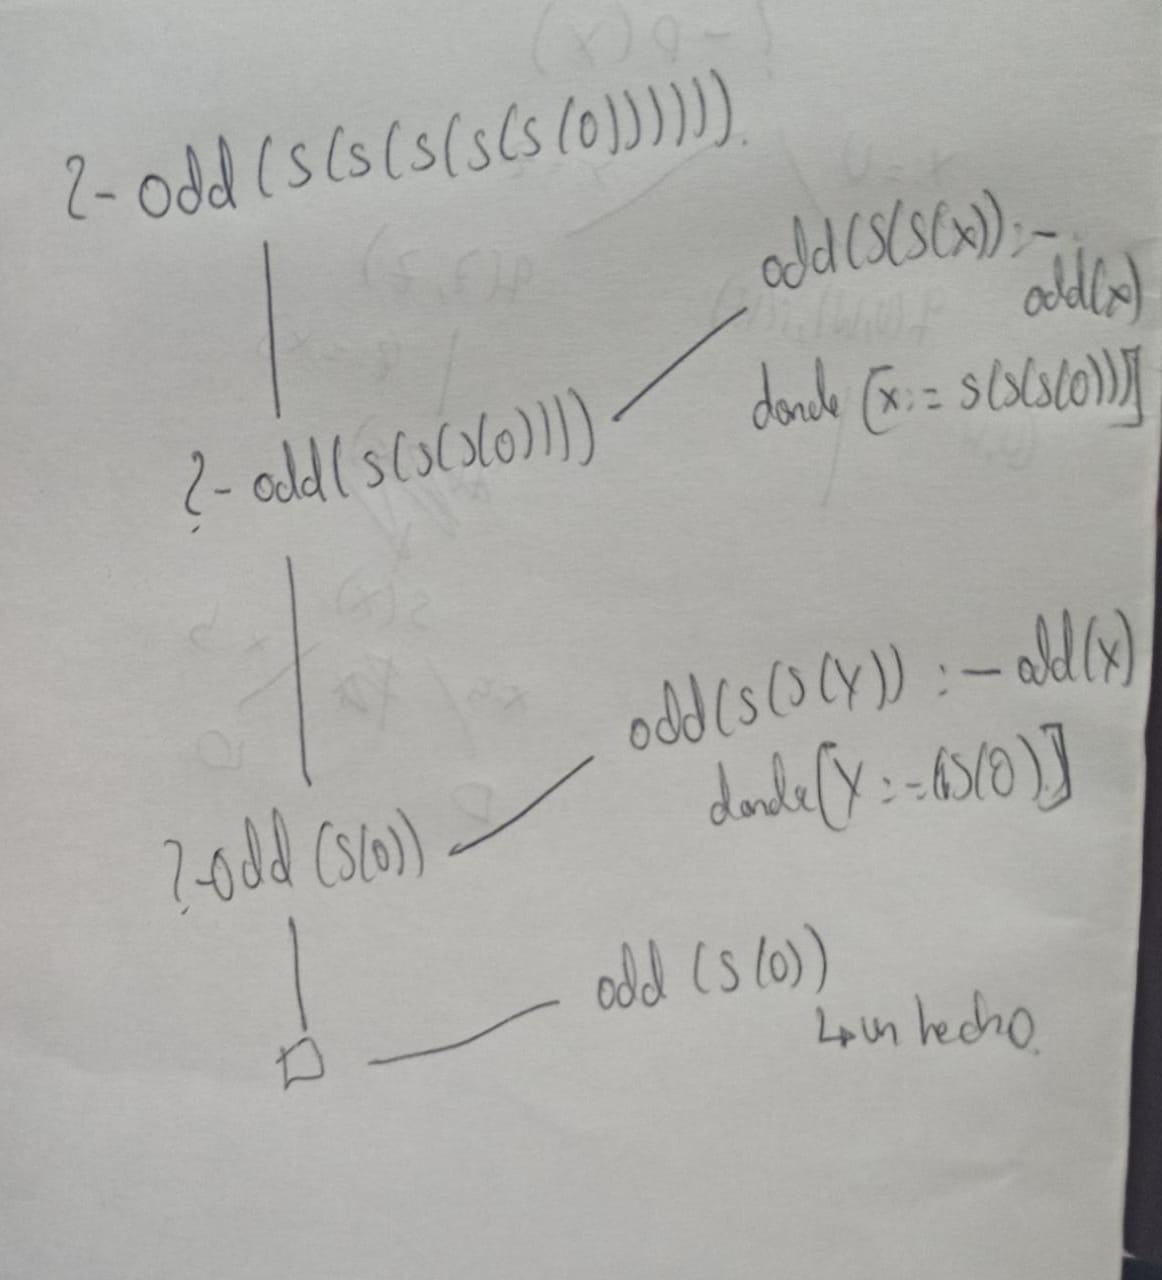
\includegraphics[scale=0.25]{4}
\end{center}

(No pude hacer que las aristas fueran para arriba, una disculpa).


\newpage
%%% 5
\item (\textbf{2pts}) 
Considera el siguiente programa lógico $\P$:
\begin{verbatim}
1.  s(a).
2.  s(b).
3.  p(U) :- q(U,W),r(W).
4.  p(Z) :- q(Z,Z).
5.  q(X,X):- s(X).
4.  r(L):- q(L,R).
\end{verbatim}
Muestre el árbol de búsqueda para la meta $G =?.-p(Y)$.

\hfill\break
 %% ARBOL
Tuve problemas para ponerle texto a las aristas, trate
de hacerlos con tikz como en los examenes pasados
pero no pude. Si tienen alguna sugerencía por favor
comentenla aquí. De nuevo una disculpa, les adjunto imagen:

\begin{center}
  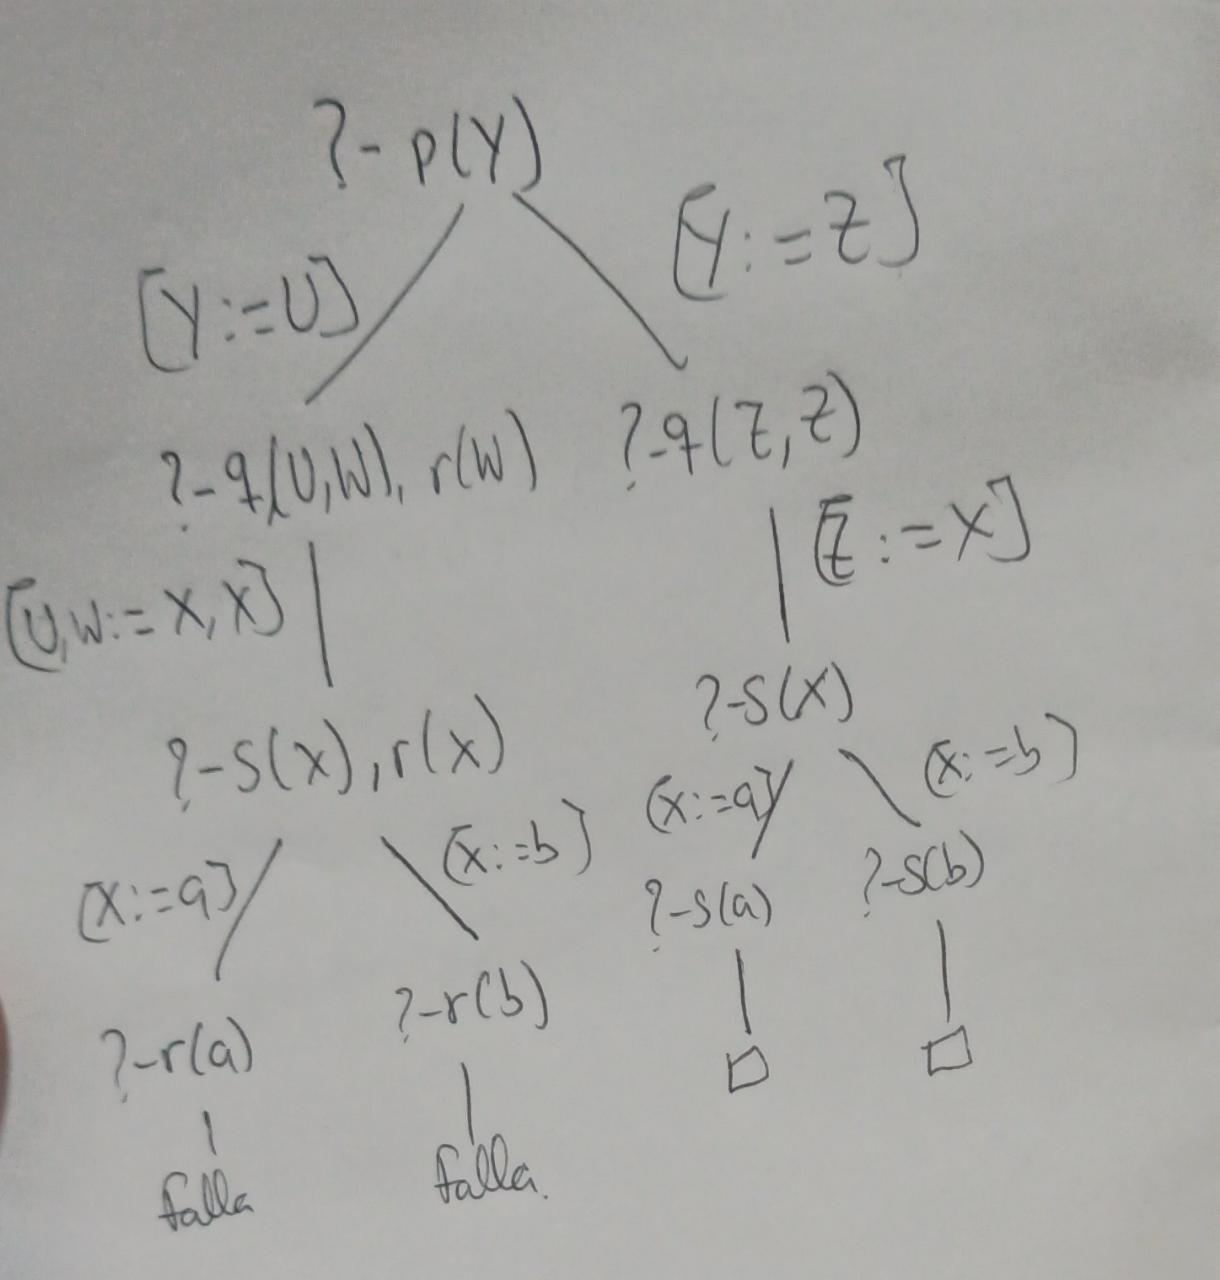
\includegraphics[scale=0.25]{5}
\end{center}

\item ({\bf Extra:
    hasta 2pts.}) Verifique la validez del siguiente argumento mediante
  resolución binaria, donde $f^{(2)},g^{(1)}$:
\[
\ba{l}
Lfxygz \lor \neg Lyz \\
\neg L fxfcfdaw \\
\hline 
\therefore \neg Lab 

\ea
\]

\item ({\bf Rescate del parcial 2 (hasta 2 puntos)}) Sean $\mathcal{L}=\{P^{(2)},\;R^{(1)},\;h^{(1)}\}$ y $\mathcal{M}=\pt{M,\I}$ donde $M=\{a,b,c\}$ y
\bi
\item[] $\mathcal{P}^\I=\{(a,b),(a,a),(b,b),(c,b)\}$
\item[] $\mathcal{R}^\I=\{a,c\}$
\item[] $h^\I(a)=b,\;h^\I(b)=b,\;h^\I(c)=a$
\ei
\begin{enumerate}
\item Decidir si  $\M\models_\sigma \fa x( Pxy \to \neg Rhx)$  donde $\sigma(y)=a $
\item Hallar un estado $\sigma$ tal que $\M\models_\sigma Pxhx \land (Rx\to Ry) $
\item Decidir si $\M\models \fa x ( Rx \to \exists y (Pxhy \land Pxy))$
\end{enumerate}

\end{enumerate}


\end{document}
